\section{Error analysis}
\label{sec:err}

Errors are signed relative errors $(\mathrm{ML}-\mathrm{SPICE})/\mathrm{SPICE}$ unless marked absolute. Figure~\ref{fig:errT} shows them against temperature and Figure~\ref{fig:worst} lists the worst rows.

\textbf{Where the errors are.}
\begin{itemize}
\item \emph{Case.} OR2 00 holds 15 of the 20 worst gate rows (largest: 4.23\% at corner 94, $T=\SI{124.5}{\celsius}$). AND2 11, 01 and 10 follow (mean signed error about $-0.2$\%) (Table~\ref{tab:worst}). At transistor level the weakest cases are OFF $I_d$, $I_s$ and $I_b$ (Table~\ref{tab:term}), and in the 100 worst gate rows the OFF devices carry 60\% of the predicted leakage, against 38\% over all rows.
\item \emph{Temperature.} The Spearman correlation between signed error and temperature is $-0.40$ for gates and $-0.745$ for the circuit. The mean signed gate error goes from $+0.20$\% below \SI{0}{\celsius} to $-0.35$\% above \SI{100}{\celsius}. The circuit goes from $+0.32$\% to $-1.01$\% (Table~\ref{tab:decomp}), and its median absolute error from 0.35\% to 0.99\%. ML under-predicts when hot. All 20 worst circuit rows are at corner 94 ($-2.9$ to $-3.1$\%).
\item \emph{Process parameters.} They matter little. The largest Spearman correlations with absolute error are VDD (0.20) and NMOS vth0 ($-0.11$) for gates, and temperature (0.39), NMOS vth0 ($-0.22$) and VDD (0.17) for the circuit; all others are below 0.12 in magnitude. Lower vth0 (more leakage) gives slightly larger errors, but vth0 is not a failure axis, and corner 94 also has a near-minimum vth0 of 0.321 V.
\end{itemize}

\begin{figure}[H]
\centering
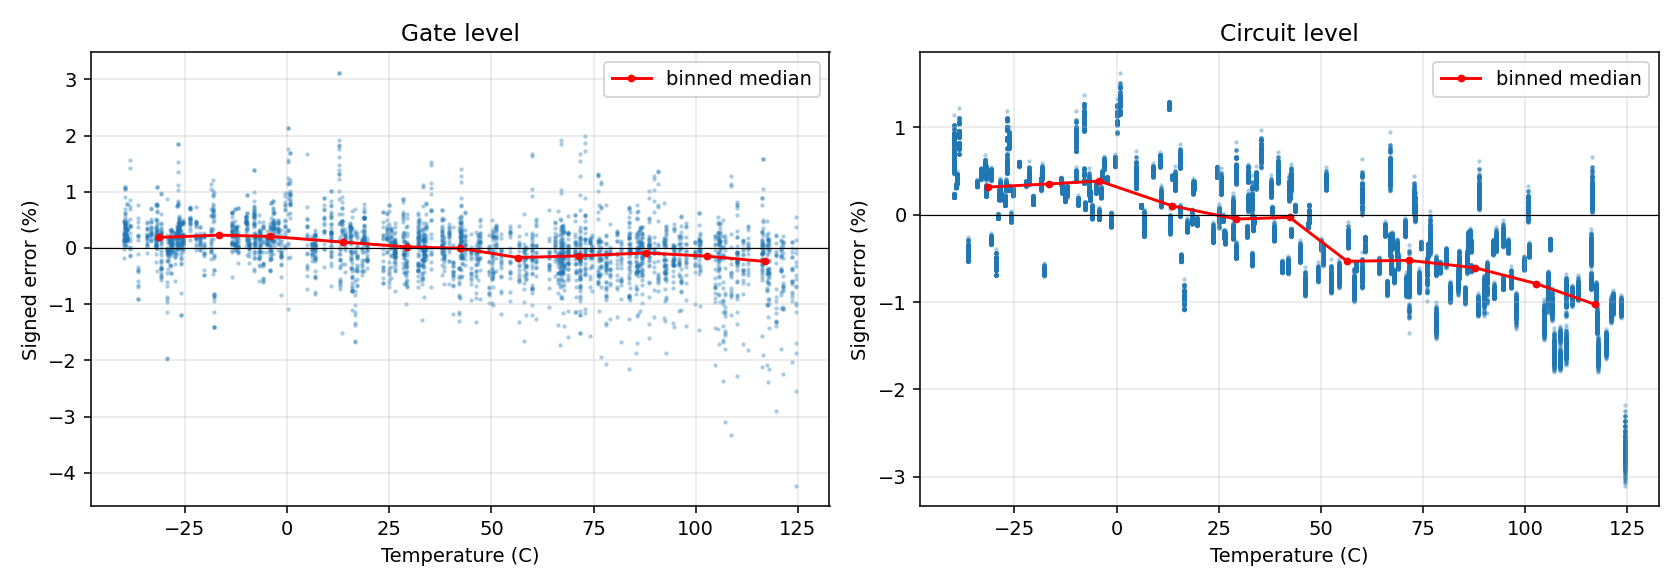
\includegraphics[width=\linewidth]{figures/analysis/error_vs_temperature.png}
\caption{Signed error against temperature for gates (left) and the circuit (right); the line is the binned median.}
\label{fig:errT}
\end{figure}

\begin{figure}[H]
\centering
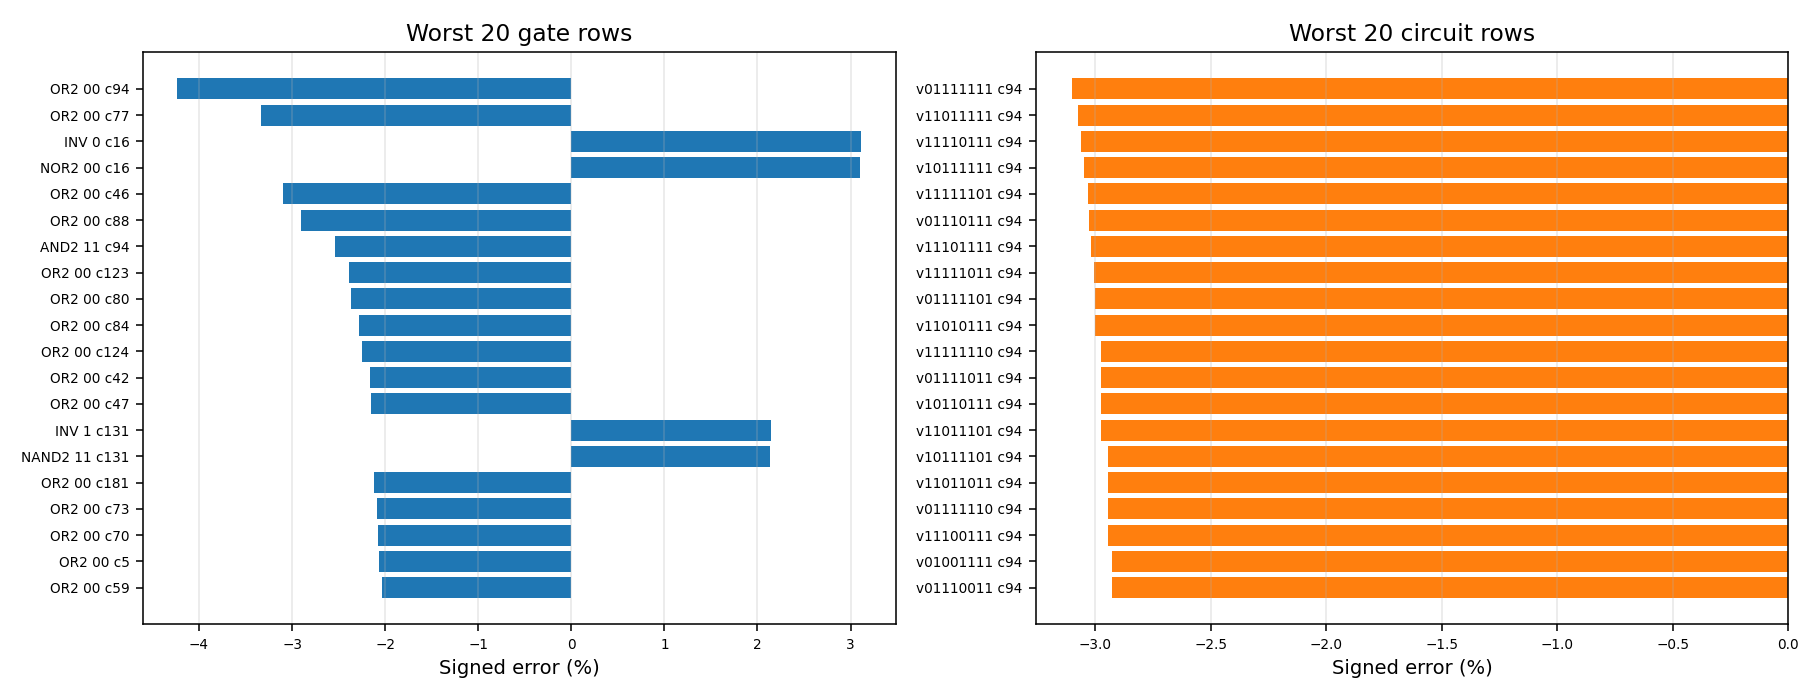
\includegraphics[width=\linewidth]{figures/analysis/worst_cases_bar.png}
\caption{The 20 worst gate rows (left) and circuit rows (right). Labels give case and corner.}
\label{fig:worst}
\end{figure}

\begin{table}[H]
\centering
\small
\caption{Gate cases with the largest errors (\%), over 200 corners. The last column is an estimate, not a SPICE result.}
\label{tab:worst}
\resizebox{\ifdim\width>\linewidth\linewidth\else\width\fi}{!}{%
\begin{tabular}{lrrrrrr}
\toprule
Case & Median abs & p95 abs & Mean signed & Max abs & Spearman (signed, $T$) & Mean signed, Vg-corrected (est.) \\
\midrule
OR2 00 & 0.709 & 2.12 & -0.764 & 4.23 & -0.85 & +0.128 \\
AND2 11 & 0.439 & 1.31 & -0.205 & 2.54 & -0.67 & +0.207 \\
AND2 01 & 0.334 & 0.94 & -0.202 & 1.69 & -0.70 & +0.143 \\
INV 0 & 0.313 & 1.14 & +0.043 & 3.12 & -0.36 & +0.043 \\
NOR2 10 (most accurate) & 0.172 & 0.77 & +0.075 & 1.57 & -0.29 & +0.075 \\
\bottomrule
\end{tabular}%
}
\end{table}


\textbf{Why OR2 00 and AND2 are worst: the OFF models never see $V_g$ off the rail.} The assigned OFF datasets fix $V_g=V_b$. The OFF models take $V_g-V_b$ as an input, but it is constant in training, so they cannot learn how the current changes when the gate moves off the rail. In AND2 and OR2, the OFF transistor of the output inverter has its gate on the internal node $z$, which sits a few millivolts off the supply rail because of the first-stage leakage (OR2 00: median 1.3 mV, up to 9 mV at hot corners). In weak inversion the current scales as $\exp(\Delta V/(nkT/q))$ for a gate offset $\Delta V$ towards turn-on. The ML model predicts the current as if the gate were exactly on the rail, so it under-predicts. A fresh single-transistor SPICE run at OR2 00, corner 94 ($z=V_{DD}-\SI{8.95}{\milli\volt}$) gives the inverter PMOS $I_d=\SI{4.306e-7}{\ampere}$ at its recorded bias. A manual ngspice 42 check of the same device with $V_g=V_{DD}$ gave \SI{3.6725e-7}{\ampere}, and ML gives \SI{3.671e-7}{\ampere}. The missing \SI{6.3e-8}{\ampere} is \SI{4.0}{\percent} of the gate leakage. The model error of this one device contributes $-4.00$ of the $-4.23$ percentage points of gate error (95\%; Table~\ref{tab:attr}). The error grows with temperature because the device leakage rises with $T$. Within OR2 00, the signed error correlates with the offset at $-0.67$.

To check this on all 200 corners we re-simulated single transistors in ngspice 42 at the exact biases recorded inside the gates (429 runs; 12 stored training rows were reproduced to within $1.1\times10^{-17}$\,A; \texttt{results/error\_analysis.json}). Moving only the gate of the OR2 00 output-inverter PMOS from its actual value back to $V_{DD}$ (offset median \SI{1.31}{\milli\volt}, maximum \SI{8.95}{\milli\volt}) lowers its true leakage power by a median of 2.70\% and up to 17.17\%. The model's median error on this device is $+0.05$\% at the rail bias it was trained on but $-2.76$\% at the actual bias. The offset grows with temperature (Spearman 0.64).

\begin{table}[H]
\centering
\small
\caption{Per-device attribution of the five worst gate rows from single-transistor SPICE at the recorded biases. Contributions are percentage points (pp) of the gate error; the last three columns sum to the gate error.}
\label{tab:attr}
\resizebox{\ifdim\width>\linewidth\linewidth\else\width\fi}{!}{%
\begin{tabular}{lrrlrrr}
\toprule
Gate / corner & $T$ (\si{\celsius}) & Gate error (\%) & Dominant OFF device(s) & Dominant (pp) & Other OFF (pp) & ON (pp) \\
\midrule
OR2 00 / 94 & 124.5 & $-4.23$ & output-inverter PMOS & $-4.00$ & $-0.14$ & $-0.09$ \\
OR2 00 / 77 & 108.5 & $-3.33$ & output-inverter PMOS & $-2.99$ & $-0.23$ & $-0.11$ \\
INV 0 / 16 & 12.8 & $+3.12$ & NMOS & $+3.05$ & $0.00$ & $+0.07$ \\
NOR2 00 / 16 & 12.8 & $+3.11$ & both NMOS & $+3.04$ & $0.00$ & $+0.07$ \\
OR2 00 / 46 & 107.1 & $-3.09$ & output-inverter PMOS & $-2.02$ & $-1.08$ & $+0.01$ \\
\bottomrule
\end{tabular}%
}
\end{table}


At corner 46 the output-inverter PMOS explains two thirds of the error; the other third comes from the two first-stage OFF NMOS, whose gates are exactly at the rail (device error $-2.5$\% each), so this row combines the gate-offset effect with ordinary OFF-model error. In all five rows the OFF devices carry 97 to 100\% of the error.

As an estimate only (not a SPICE result), a first-order correction $\exp(\Delta V/(nkT/q))$ with $n=1.64$ calibrated on that one check reduces the OR2 00 mean signed error from $-0.76$\% to $+0.13$\% (last column of Table~\ref{tab:worst}). Over all gate rows it would lower the p95 error from 1.12\% to 0.90\% and the maximum from 4.23\% to 3.12\%.

The remaining worst gate rows have the opposite sign. INV 0 and NOR2 00 at corner 16 ($T=\SI{12.8}{\celsius}$) over-predict by $+3.1$\%. The OFF NMOS carries 68.5\% of the leakage, has its gate exactly at 0~V and is over-predicted by 4.44\% (Table~\ref{tab:attr}). This is a rare local outlier of the NMOS OFF model, not the gate-offset effect: on the 15,000 held-out NMOS OFF rows the power error has p95 0.48\% and p99 1.17\%, and only 4 rows exceed 4.4\%. The corner combines thin NMOS oxide (14.5th percentile) with high $V_{DD}$ (93rd percentile); we did not isolate which one causes the outlier.

\textbf{Circuit: composition is the main hot-corner error.} The circuit prediction sums standalone gate predictions. The stored sum of the true standalone SPICE gate leakages lets us split the circuit error into two parts (Table~\ref{tab:decomp}). Above \SI{100}{\celsius}, the sum of standalone SPICE gate leakages is already $-1.04$\% below the full-circuit SPICE, while ML differs from that SPICE gate sum by only $+0.03$\%. So the hot-corner circuit error comes from composing ideal standalone gates, not from ML: inside the circuit each NAND2 is driven by another gate's output rather than by an ideal rail, and the slightly off-rail inputs raise the leakage of the OFF devices, more so at high temperature. An exact gate model would therefore still under-predict by about 1\% at hot corners. At the worst circuit row (vector 01111111, corner 94) the standalone-sum error is $-2.84$\% and the ML-versus-sum error is $-0.26$\% (both relative to the full-circuit SPICE, so they add up to $-3.10$\%). At cold corners the opposite holds: the composition error is near zero and ML contributes $+0.24$\%.

\begin{table}[H]
\centering
\small
\caption{Mean signed circuit error (\%) by temperature band.}
\label{tab:decomp}
\resizebox{\ifdim\width>\linewidth\linewidth\else\width\fi}{!}{%
\begin{tabular}{lrrrr}
\toprule
$T$ band ($^\circ$C) & Rows & ML vs full SPICE & Standalone sum vs full SPICE & ML vs standalone sum \\
\midrule
$-40$ to 0 & 14,592 & +0.32 & +0.07 & +0.24 \\
0 to 25 & 6,400 & +0.23 & -0.02 & +0.25 \\
25 to 50 & 8,448 & -0.04 & -0.16 & +0.12 \\
50 to 75 & 7,936 & -0.42 & -0.44 & +0.02 \\
75 to 100 & 7,680 & -0.61 & -0.65 & +0.04 \\
100 to 125 & 6,144 & -1.01 & -1.04 & +0.03 \\
\midrule All & 51,200 & -0.16 & -0.30 & +0.13 \\
\bottomrule
\end{tabular}%
}
\end{table}


\textbf{Numerical validation.} The predicted four-current KCL residual of the gate-device queries has a median of $7.57\times10^{-18}$\,A and a maximum of $1.31\times10^{-12}$\,A. No clipping is applied, and none of the FET predictions or whole-gate predictions has negative calculated power (\texttt{results/hierarchy\_summary.json}). Source closure gives per-device current conservation for the energy calculation, but it does not enforce passivity or node balance between devices. Independent checks of the SPICE references (\texttt{reports/circuit\_reference\_validation.json}, \texttt{code/scripts/verify\_circuit\_references.py}) use separate terminal ammeters and manually assembled gate references to compare transistor dissipated power with the power of the external sources, and add reverse-order and fresh-input parity checks. All of them passed.
